\documentclass{article}
\usepackage[utf8]{inputenc}
\usepackage{graphicx}
\usepackage{tikz}
\usepackage{float}
\usetikzlibrary{positioning,fit,calc,arrows.meta, shapes}
\graphicspath{ {images/} }

%Tot això hauria d'anar en un pkg, però no sé com és fa
\newcommand*{\assignatura}[1]{\gdef\1assignatura{#1}}
\newcommand*{\grup}[1]{\gdef\3grup{#1}}
\newcommand*{\professorat}[1]{\gdef\4professorat{#1}}
\renewcommand{\title}[1]{\gdef\5title{#1}}
\renewcommand{\author}[1]{\gdef\6author{#1}}
\renewcommand{\date}[1]{\gdef\7date{#1}}
\renewcommand{\maketitle}{ %fa el maketitle de nou
    \begin{titlepage}
        \raggedright{UNIVERSITAT DE LLEIDA \\
            Escola Politècnica Superior \\
            Grau en Enginyeria Informàtica\\
            \1assignatura\\}
            \vspace{5cm}
            \centering\huge{\5title \\}
            \vspace{3cm}
            \large{\6author} \\
            \normalsize{\3grup}
            \vfill
            Professorat : \4professorat \\
            Data : \7date
\end{titlepage}}
%Emplenar a partir d'aquí per a fer el títol : no se com es fa el package
%S'han de renombrar totes, inclús date, si un camp es deixa en blanc no apareix

\tikzset{
	%Style of nodes. Si poses aquí un estil es pot reutilitzar més facilment
	pag/.style = {circle, draw=black,
                           minimum width=0.75cm, font=\ttfamily,
                           text centered}
}
\renewcommand{\figurename}{Figura}
\title{Laboratori 5}
\author{Sergi Sales Jové, Sergi Simón Balcells}
\date{Dimarts 19 de Novembre}
\assignatura{Estructures de dades}
\professorat{X. Domingo, J.E. Garrido, JM. Gimeno}
\grup{GM3}

%Comença el document
\begin{document}
\maketitle
\thispagestyle{empty}

\newpage
\pagenumbering{roman}
\tableofcontents
\newpage
\pagenumbering{arabic}

\section{Introducció}
L'objectiu del projecte és crear un prototip a paper de l'aplicació
EcoScanner i explicar les decisions de disseny resultants. S'ha utilitzat la
tècnica de prototipat de baixa fidelitat, amb el fi de poder posar
sobre la taula totes les oportunitats de disseny plantejades en l'anàlisi
de requisits.\\
\\
Utilitzar aquest tipus de tècniques proporciona una forma flexible i visual
amb la que començar a treballar de forma senzilla i econòmica en la part
de la interfície i la interacció amb les funcionalitats de l'aplicació.\\
\\
La intenció d'aquest projecte és proposar una interfície per l'aplicació
i comprovar si els usuaris són capaços de saber què fer i com interactuar
amb ella. Així, serà possible trobar elements que inicialment
semblaven intuïtius pels desenvolupadors de l'aplicació, però realment
complicats o antiintuïtius pels usuaris reals. \\
%
\section{Usabilitat General}
Seguint les indicacions de l'anàlisi de requisits, s'ha prioritzat una
sèrie de qualitats a l'hora del disseny de la interfície, entre
elles la rapidesa.
És per això que l'aplicació facilita la funcionalitat principal,
l'escàner de productes, fins al punt que s'arriba a ella amb
només un clic.
\\\\
S'ha optat per un disseny lleuger, amb pocs elements a interactuar
per pantalla, amb aquests sent grans i vistosos, mantenint una informació
mínima i justa per evitar la saturació de l'usuari.
\\\\
S'ha utilitzat una sèrie de normes de consistència per facilitar el procés
d'aprenentatge. Per exemple, la major part de botons i elements
interactius són de color verd, d'aquesta forma s'aconsegueix que l'usuari
relacioni el color verd amb un element interactiu. Un altre
exemple és l'ús del mateix disseny de fletxa verda i de forma
arrodonida, per retornar a la
pantalla anterior.

\section{Pantalla principal}
En la primera pantalla (o menú), es troba el botó per accedir a la
funcionalitat principal de l'aplicació, l'escàner de productes. Aquest
botó és l'element més destacat de la pantalla, ocupant la major part
d'ella. És de color verd, com la resta d'elements interactius de l'app
i hi apareix el logotip d'EcoScanner, un arbre. La interacció amb el botó
és mitjançant un clic, i porta a la pantalla d'escàner (2).\\
\\
A sota d'aquest hi ha un requadre on apareix la
vista prèvia de curiositats, notícies i esdeveniments d'interès relacionats
amb EcoScanner i el món del reciclatge en general. S'hi pot interactuar
prement a sobre, i porta a la pantalla de notícies (4).\\
\\
Al peu de la pantalla principal es troba el botó per
anar a la pantalla de configuració (5). El botó és un cercle que conté
el dibuix d'un engranatge minimalista. Aquest és així, ja que
les aplicacions acostumen a utilitzar-ho, fent que sigui més
fàcil de reconèixer la seva utilitat.\\
\\
Els dos últims elements interactius de la pantalla principal són per
recolzar el sistema de navegació per "swipe" de la pantalla principal. El
primer és una silueta d'una persona, fa la mateixa funcionalitat que un swipe
a l'esquerra, porta a la pantalla de "les meves captures" (6). El segon és
una xinxeta d'ubicació, fa la mateixa funció que un swipe a la dreta, porta a
la pantalla dels contenidors més propers (9).\\
\\
L'aprenentatge dels swipe es donarà per animacions si es clica el botó,
o sigui, es mostri com es llisca la pantalla, i tres puntets superiors,
només pintat el del mig. Aquest element és àmpliament utilitzat tant en
aplicació com en els mateixos sistemes operatius, fent que sigui reconeixible.
\\\\

\section{Escàner}
% pagina 2

En la segona pantalla es troba un únic botó, aquest
és un botó de retorn el qual portarà
al menú (1). Un cop escanejat un codi de barres es reencaminarà
a la pantalla on es mostren els detalls del producte que es vol reciclar. (3)
\\\\
% Pagina 3
En la tercera pantalla s'hi troben dos elements d'interacció.
Un és un botó de retorn que porta al menú (P1)
si l'usuari prové de la segona pantalla i anirà a
la pantalla 7 i 8 si prové d'aquestes. L'altre
element d'interacció és un botó arrodonit de color
verd que es troba a la part inferior del mapa, amb el text
"Contenidors més propers". Aquest, porta a la pantalla 10.
A la part de dalt de la pantalla, es mostren
en requadres amb imatges els elements de l'objecte
que es vol reciclar i a quin contenidor ha d'anar cada un d'ells.
Com ha afegit es mostra al peu de cada imatge el nom de l'element i el contenidor.

\section{Els Meus escanejos}
En la sisena pantalla s'ofereix informació el nombre
d'escanejos que ha realitzat l'usuari
així com del top tres d'articles més escanejats.
A més, es pot interactuar amb aquests 4 elements fent clic,
per remarcar-ho se'ls hi ha donat el característic color verd
a més de la forma de cercle, com al botó principal del menú (1).
Finalment, aquests elements porten a la pantalla 7 al clicar al botó
de l'apartat "Els Meus Escanejos", i a la pantalla 8 en
cas de fer clic a qualsevol dels elements de l'apartat
"Els Més Escanejats".
Per a retornar a la pantalla del menú (1), com que es mostra
la transició per arribar a aquesta, els botons de suport
del swipe no es mostren. Per tant només es podrà
retornar fent swipe a l'esquerra.
\\\\
%Pagina 7
%
Aquesta pantalla conté un llistat dels escanejos més recents
que ha realitzat l'usuari. Si es vol tornar a consultar
algun element que prèviament escanejat, es pot fer de forma senzilla
sense la necessitat de tornar-ho a fer.
\\\\
En aquesta interfície es pot
interactuar de tres maneres diferents. Una d'elles és
el botó de retorn de dalt a l'esquerra,
la qual porta al menú "Les Meves Captures" (6). També es pot fer scroll
cap amunt i cap a baix per tal de veure tots els elements escanejats, a mesura que
es fa l'scroll cap a baix es van carregant els elements escanejats.
Finalment, es pot clicar a un dels elements de la llista, el qual
et porta a la pàgina amb la informació d'on ha d'anar reciclada cada una
de les parts del producte (3).
\\\\
% Pagina 8
%
En aquesta pantalla apareixen dos elements d'interacció
diferents. El primer és un botó de retorn amb
el títol de la pantalla: "Els Més Escanejats".
El segon element interactiu son cada un
dels articles més escanejats per ordre,
amb un botó que els porta a la pàgina de detalls (3) de
l'element amb qüestió. Com a element clicable és de color
verd, a més a més de ser de forma circular. El botó de
retorn torna a la pantalla (6).
%\\\\
\section{Contenidors més propers}
% pàgina
La segona funcionalitat més important és la d'indicar els contenidors més
propers a l'usuari. És per això que està només a un swipe esquerra de la
pantalla principal (1). Aquesta funcionalitat consta de dues pantalles,
la previsualització (9) i el mapa (10).\\
\\
Fent un swipe a l'esquerra des de la pantalla principal s'accedeix a la
pantalla de previsualització del mapa. Aquesta és molt simple i fa la
funció d'intermediari entre la pantalla principal i el mapa complet amb
totes les funcionalitats. Consta només d'un requadre amb la vista prèvia
del mapa amb els contenidors disponibles i a sobre un text que hi fica
"Contenidors més propers".\\
\\
El requadre de la vista prèvia del mapa, a l'aparèixer-hi un plànol, és un
element interactiu que no està pintat de verd, patró que segueix la
majoria d'elements interactius. Per donar a veure què es pot clicar,
aquest element fa una animació d'expansió i contracció molt minimalista.
Una vegada clicat, s'expandeix del tot i apareix la pantalla del mapa (10).
\\\\
%Pàgina 10
%
En la pantalla del mapa (10) apareix un plànol on està indicada la ubicació
de l'usuari i els contenidors més propers. En la part inferior de la pantalla
hi ha un requadre amb els contenidors més importants. L'usuari pot seleccionar
o desseleccionar els contenidors en funció de si li interessa o no veure'ls al
mapa. Com que al mapa s'hi pot accedir des de 2 pantalles diferents, la immediata
a escanejar un producte (3) i la dels elements més buscats (9), els contenidors
que vindran prèviament seleccionats variaran en funció de la pantalla que vingui.
El mapa, com ja és habitual en els dispositius mòbils es podrà moure lliscant
amb el dit.

A més a més, hi haurà una fletxeta cap a dalt com un signe de potència
($\wedge$). Aquest element, en arrossegar-se (swipe), desplegarà un petit
menú en forma de quadrícula d'elements per poder seleccionar entre una
varietat més gran de contenidors i altres ubicacions de reciclatge.
\\\\
La fletxa cap amunt ve recolzada en les últimes
actualitzacions d'Android, on l'utilitzen per a ensenyar-te
totes les aplicacions a la pantalla principal, fent que per
la majoria dels usuaris sigui un element ja reconegut.
\\\\
En desplegar-se el menú, la mateixa fletxa apuntarà cap a
baix, que indicarà com tancar-ho. També apareixerà mínimament
la silueta del mapa, i, com els menús arrossegables ja vists en els
moblis, tant si es clica el mapa com es llisca cap a baix es
tancarà el menú.
\\\\
En aquest menú, els contenidors no seleccionats apareixeran en un fons verd,
i significaria que poden ser clicats. Els que ja han estat seleccionats
apareixen en taronja (colors triada).

Tot i que el color taronja no s'hagi vist massa en l'aplicació,
el color verd, que fins ara s'ha utilitzat per elements interactius,
hauria de facilitar l'aprenentatge de l'usuari. En veure que
quan clica el contenidor que vol cercar, canvia de color, intueixi que
ha estat seleccionat. \\\\
%
A dalt del requadre apareixen dos elements: una lupa i un "Marcar tots" amb
un petit requadre al costat. El primer element servirà per
facilitar la cerca del contenidor desitjat. El segon servirà per a marcar
tots els tipus de contenidors a la vegada. Si l'usuari clica aquest, veurà
tots els requadres de color taronja, i també com apareixen tots els contenidors
en el mapa, a més d'un tic en el petit requadre de "Marcar tots".
%\\\\
% Descomentar si no és l'últim paràgraf.

\section{Extres}
En aquesta secció es recull aquelles pantalles que no formen part d'un conjunt amb una funcionalitat comuna, sinó que són pantalles individuals amb la seva propia funció.
\subsection{Configuració}
En aquesta pantalla es podràn configurar 
diverses opcions relacionades amb l'usabilitat 
que tindrà l'aplicació, com per 
exemple la vibració al final d'un escaneig, 
si es vol activar la localització o no...
Conté 3 elements interactius diferents, 
els tres seleccionadors horitzontals 
tenen la funció d'habilitar i deshabilitar les 
opcions que s'especifiquen al seu cantó. 
Els altres dos elements, que es troben al peu de la pantalla,
són dos desplegables els quals s'hi pot interactuar fent click. Quan es clica
s'inicia una animació de desplegament cap amunt fins a aproximadament
mitja pantalla, on en el cas de suport hi apareixen els camps a omplir
per contactar amb els desenvolupadors i, en el cas d'About, un petit text donant 
informació sobre l'aplicació i l'empresa.

\subsection{Notícies}
% pàgina 4
La pantalla de notícies té dos elements interactius, el 
primer és el botó de retorn que porta a la pantalla principal (1).
El segon element és el suport visual del swipe ja
vist en la pantalla del menú (1), que en aquest cas serveix per navegar per
les notícies.

\\\\

\section{Graf de navegabilitat}
<<<<<<< HEAD

=======
S'ajunta un graf representant les pantalles i 
a on es poden dirigir per a facilitar la compresió.
>>>>>>> 427edfb52e010a24c1bc0829d0b569b75b737fe4
%Especificar disseny de lletres
%Si s'accedeix a la pantalla 3 des de la pantalla 7, dir que el botó de retorn
%torna la pantalla 3

%Al prototip, assumpte va amb p lmao

\begin{figure}[H]
    \centering
    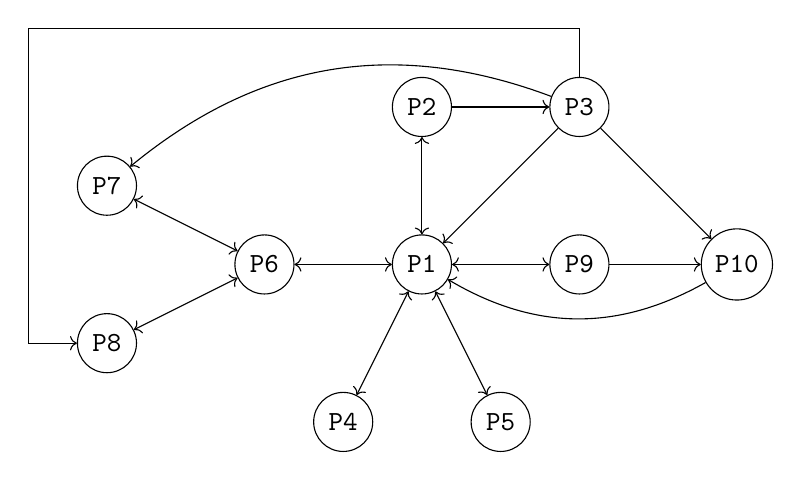
\begin{tikzpicture}
    	%nodes
    	\node[pag] (1)  at (4, 2) {P1};
    	\node[pag] (2)  at (4, 4) {P2};
    	\node[pag] (3)  at (6, 4) {P3};
    	\node[pag] (4)  at (3, 0) {P4};
    	\node[pag] (5)  at (5, 0) {P5};
    	\node[pag] (6)  at (2, 2) {P6};
    	\node[pag] (7)  at (0, 3) {P7};
    	\node[pag] (8)  at (0, 1) {P8};
    	\node[pag] (9)  at (6, 2) {P9};
    	\node[pag] (10) at (8, 2) {P10};
    	%arrows
    	\draw[<->] (1)  edge (2)
    			   (1)  edge (4)
    			   (1)  edge (5)
    			   (1)  edge (6)
    			   (1)  edge (9)
    			   (6)  edge (7)
    			   (6)  edge (8);
    	\draw[->, bend left]  (10) edge (1);
    	\draw[->, bend right] (3)  --   (6, 5) -- (-1, 5) -- (-1, 1) -- (8);
    	\draw[->, bend right] (3)  edge (7);
    	\draw[->]  (2)  edge (3)
    			   (3)  edge (1)
    			   (3)  edge (10)
    			   (9)  edge (10);
    	

    \end{tikzpicture}
    \caption{Graf de representació de navegabilitat de pantalles}
    \label{grp:map}
\end{figure}

\end{document}
